\documentclass[tikz,border=6pt]{standalone}
\usetikzlibrary{arrows.meta}
\definecolor{ink}{HTML}{E6EDF3}
\definecolor{gapfill}{HTML}{30363D}
\definecolor{innerfill}{HTML}{0D1117}
\begin{document}
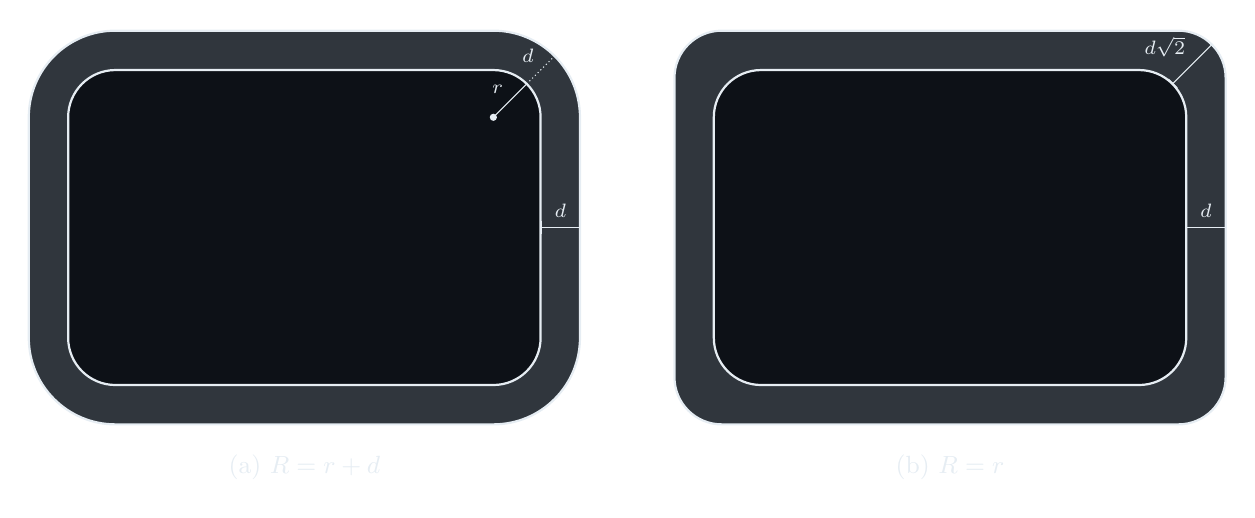
\begin{tikzpicture}[color=ink]
  \begin{scope}
    \fill[gapfill, rounded corners=1.1cm] (-3.5,-2.5) rectangle (3.5,2.5);
    \draw[thick, rounded corners=1.1cm] (-3.5,-2.5) rectangle (3.5,2.5);
    \fill[innerfill, rounded corners=0.6cm] (-3,-2) rectangle (3,2);
    \draw[thick, rounded corners=0.6cm] (-3,-2) rectangle (3,2);
    \fill[ink] (2.4,1.4) circle (1.3pt);
    \draw[thin] (2.4,1.4) -- (2.824,1.824)
      node[midway, above left=-1pt, font=\scriptsize] {$r$};
    \draw[thin, densely dotted] (2.824,1.824) -- (3.178,2.178)
      node[midway, above left=-1pt, font=\scriptsize] {$d$};
    \draw[|-|, thin] (3.0,0) -- (3.5,0) node[midway, above, font=\scriptsize] {$d$};
    \node[font=\small] at (0,-3.05) {(a) $R = r + d$};
  \end{scope}
  \begin{scope}[xshift=8.2cm]
    \fill[gapfill, rounded corners=0.6cm] (-3.5,-2.5) rectangle (3.5,2.5);
    \draw[thick, rounded corners=0.6cm] (-3.5,-2.5) rectangle (3.5,2.5);
    \fill[innerfill, rounded corners=0.6cm] (-3,-2) rectangle (3,2);
    \draw[thick, rounded corners=0.6cm] (-3,-2) rectangle (3,2);
    \draw[|-|, thin] (3.0,0) -- (3.5,0) node[midway, above, font=\scriptsize] {$d$};
    \draw[|-|, thin] (2.824,1.824) -- (3.324,2.324)
      node[midway, above left=-1pt, font=\scriptsize] {$d\sqrt2$};
    \node[font=\small] at (0,-3.05) {(b) $R = r$};
  \end{scope}
\end{tikzpicture}
\end{document}
